\tikzstyle{box} = [rectangle, minimum width=3cm, minimum height=1cm, text centered, draw=black]
\tikzstyle{arrow} = [thick,->,>=stealth]

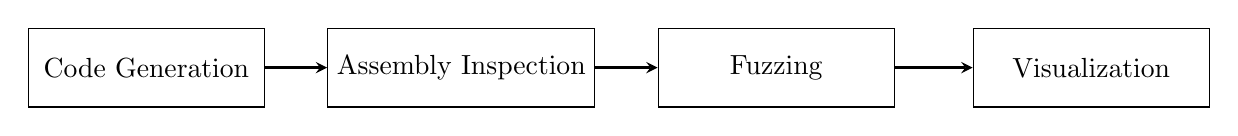
\begin{tikzpicture}
  \node (Code Generation) [box] {Code Generation};
  \node (Assembly Inspection) [box, right of=Code Generation, xshift=3cm] {Assembly Inspection};
  \node (Fuzzing) [box, right of=Assembly Inspection, xshift=3cm] {Fuzzing};
  \node (Visualization) [box, right of=Fuzzing, xshift=3cm] {Visualization};

  \draw [arrow] (Code Generation) -- (Assembly Inspection);
  \draw [arrow] (Assembly Inspection) -- (Fuzzing);
  \draw [arrow] (Fuzzing) -- (Visualization);
\end{tikzpicture}